\documentclass[aspectratio=169]{beamer}
\usetheme{Madrid}
\usecolortheme{seahorse}
\usepackage{amsmath, amssymb}
\usepackage{listings}
\usepackage{xcolor}
\usepackage{tikz}
\usetikzlibrary{arrows.meta, positioning, shapes.geometric, fit, backgrounds, decorations.pathreplacing}

\lstset{
  basicstyle=\ttfamily\small,
  commentstyle=\color{gray!70}\itshape,
  numbers=left,
  numberstyle=\tiny\color{gray},
  breaklines=true,
  frame=single,
  backgroundcolor=\color{gray!8},
  keepspaces=true,
  showstringspaces=false,
}

\title{ElasticNet Regression in Rust}
\subtitle{Jacobi Coordinate Descent — Parallelisation and Cache-Fusion Optimisations}
\author{Armin Ebrahimi Saba}
\date{\today}

% ─────────────────────────────────────────────────────────────────────────────

\begin{document}

\begin{frame}
  \titlepage
\end{frame}

\begin{frame}{Outline}
  \tableofcontents
\end{frame}

% ─────────────────────────────────────────────────────────────────────────────
\section{Objective and Problem Formulation}

\begin{frame}{ElasticNet Objective}
  \begin{block}{Minimisation target}
    \[
      \min_{w,b}\;\frac{1}{2n}\|y - Xw - b\|_2^2
      \;+\;\alpha\rho\|w\|_1
      \;+\;\frac{\alpha(1-\rho)}{2}\|w\|_2^2
    \]
  \end{block}
  \vspace{0.4em}
  \begin{columns}
    \column{0.5\textwidth}
    \begin{itemize}
      \item $\alpha$ — total regularisation strength
      \item $\rho$ (\texttt{l1\_ratio}) — Lasso/Ridge mix
      \item $\rho=1$: pure Lasso (sparsity)
      \item $\rho=0$: pure Ridge (shrinkage)
    \end{itemize}
    \column{0.5\textwidth}
    \begin{itemize}
      \item $n$ — number of training samples
      \item $w \in \mathbb{R}^p$ — coefficient vector
      \item $b$ — optional unpenalised intercept
      \item $X \in \mathbb{R}^{n \times p}$ — design matrix (C-contiguous \texttt{f32})
    \end{itemize}
  \end{columns}
\end{frame}

% ─────────────────────────────────────────────────────────────────────────────
\section{Optimisation History}

\begin{frame}{Commit-by-Commit Timeline}
  Three commits, each removing one concrete bottleneck. The following sections
  detail each in turn.
  \vspace{0.5em}
  \begin{center}\small
  \begin{tabular}{lp{5.2cm}p{4.8cm}}
    \hline
    \textbf{Commit} & \textbf{Change} & \textbf{Bottleneck solved} \\
    \hline
    \texttt{cdeb7a3} & \textbf{Jacobi} parallel coordinate descent: freeze
      $w^{(t)}$, update all $\Delta w_j$ from one frozen residual & Gauss--Seidel
      CD is serial: $2p$ barriers/iter $\Rightarrow$ can't parallelise \\[3pt]
    \texttt{0ad4263} & \textbf{Fused single-pass}: each row-block of $X$ read once
      --- phase 1 updates $r$, phase 2 accumulates $X^\top r$ (L2-hot) & Two-pass
      Jacobi read $X$ from DRAM \textbf{twice} per iteration ($\gtrsim$20 MB) \\[3pt]
    \texttt{10f16bd} & \textbf{Zero-copy} \texttt{ArrayView2} predict +
      \textbf{block-parallel} rows (L2-sized tasks) & Predict copied $X$ over FFI
      and spawned one task/row $\Rightarrow$ lost to sklearn at scale \\
    \hline
  \end{tabular}
  \end{center}
  \vspace{0.4em}
  {\footnotesize Also in \texttt{0ad4263}: exact intercept lag correction
   ($\Delta b = \overline{r} - c^\top\!\Delta w / n$) and stratum global-thread-pool
   integration. In \texttt{10f16bd}: \texttt{--large/--xlarge/--xxlarge} benchmark
   tiers.}
\end{frame}

% ─────────────────────────────────────────────────────────────────────────────
\section{Commit 1 — Jacobi Parallel Coordinate Descent}

\begin{frame}{Coordinate Descent: Core Update Rule}
  For each coordinate $j$, holding all others fixed, the unconstrained minimum
  over $w_j$ is the \emph{soft-threshold}:
  \[
    \hat{w}_j
    = \frac{S\!\left(\rho_j,\;\alpha\rho\right)}{\|X_{:j}\|^2/n + \alpha(1-\rho)}
    \qquad
    \rho_j = \frac{X_{:j}^\top r}{n} + w_j\,\frac{\|X_{:j}\|^2}{n}
  \]
  where $r = y - Xw - b$ is the residual vector and
  \[
    S(z,\,t) = \operatorname{sign}(z)\max(|z|-t,\,0)
  \]
  is the soft-threshold (proximal) operator.
\end{frame}

\begin{frame}[fragile]{Soft-Threshold Operator in Rust}
\begin{lstlisting}
fn soft_threshold(x: f32, t: f32) -> f32 {
    if      x >  t { x - t }
    else if x < -t { x + t }
    else            { 0.0   }
}
\end{lstlisting}
  \vspace{0.6em}
  The coordinate update then becomes:
\begin{lstlisting}
let rho_j   = dots[j] / n + coef[j] * col_norm_sq[j];
let new_w   = soft_threshold(rho_j, l1_pen)
              / (col_norm_sq[j] + l2_pen);
let delta   = new_w - coef[j];
coef[j]     = new_w;
\end{lstlisting}
\end{frame}

\begin{frame}{Jacobi vs.\ Gauss-Seidel Parallelism}
  \begin{columns}
    \column{0.48\textwidth}
    \textbf{Gauss-Seidel (sequential)}
    \begin{itemize}
      \item Update one $w_j$ at a time using the latest residual
      \item 2 DRAM passes per coordinate $\Rightarrow$ $2p$ barriers / outer iteration
      \item Simple but inherently serial — poor GPU/multicore fit
    \end{itemize}
    \column{0.48\textwidth}
    \textbf{Jacobi (parallel, commit 1)}
    \begin{itemize}
      \item Freeze $w^{(t)}$; compute all $\Delta w_j$ simultaneously
      \item Only \textbf{2 Rayon barriers per outer iteration} regardless of $p$
      \item \texttt{par\_chunks} fold/reduce over rows — embarrassingly parallel
      \item 2--7$\times$ faster than sklearn on $10{,}000$--$100{,}000 \times 50$--$100$
    \end{itemize}
  \end{columns}
\end{frame}

\begin{frame}[fragile]{Jacobi Two-Pass Loop (commit 1)}
  \textbf{Pass 1} — accumulate $X^\top r$ in parallel:
\begin{lstlisting}
x_raw.par_chunks(n_cols)
     .fold(|| vec![0.0f32; n_cols], |mut acc, row| {
         axpy_scalar(&mut acc, r[row_idx], row); acc
     })
     .reduce(|| vec![0.0f32; n_cols],
             |mut a, b| { for j in 0..n_cols { a[j] += b[j] } a })
\end{lstlisting}

  \textbf{Pass 2} — update residuals in parallel:
\begin{lstlisting}
r.par_chunks_mut(1).enumerate().for_each(|(i, ri)| {
    ri[0] -= dot_scalar(x_row_i, &delta_w);
});
\end{lstlisting}

  \begin{alertblock}{Bottleneck at scale}
    Both passes read all of $X$ from DRAM when the matrix exceeds L3 cache
    ($\gtrsim$20 MB). Two full reads per iteration $\Rightarrow$ memory-bandwidth bound.
  \end{alertblock}
\end{frame}

% ─────────────────────────────────────────────────────────────────────────────
\section{Commit 2 — Fused Single-Pass with Thread Pool}

\begin{frame}{Cache-Fusion Insight}
  \begin{block}{Key observation}
    After reading a row block of $X$ into L2 cache for the residual update
    (phase~1), that block is still \emph{hot} in L2.  We can immediately
    accumulate $X^\top r$ for that block (phase~2) before eviction —
    \textbf{one DRAM read instead of two}.
  \end{block}
  \vspace{0.4em}
  \begin{center}
  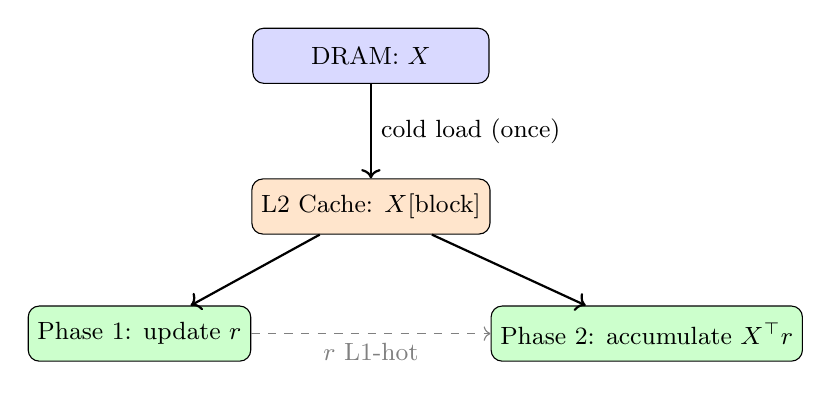
\begin{tikzpicture}[node distance=1.2cm, every node/.style={font=\small}]
    \node[draw, fill=blue!15, rounded corners, minimum width=3cm, minimum height=0.7cm] (dram) {DRAM: $X$};
    \node[draw, fill=orange!20, rounded corners, minimum width=3cm, minimum height=0.7cm, below=of dram] (l2) {L2 Cache: $X[\text{block}]$};
    \node[draw, fill=green!20, rounded corners, minimum width=2.5cm, minimum height=0.7cm, below left=0.9cm and 0cm of l2] (p1) {Phase 1: update $r$};
    \node[draw, fill=green!20, rounded corners, minimum width=2.5cm, minimum height=0.7cm, below right=0.9cm and 0cm of l2] (p2) {Phase 2: accumulate $X^\top r$};
    \draw[->, thick] (dram) -- node[right]{cold load (once)} (l2);
    \draw[->, thick] (l2) -- (p1);
    \draw[->, thick] (l2) -- (p2);
    \draw[dashed, ->, gray] (p1) -- node[below, gray]{$r$ L1-hot} (p2);
  \end{tikzpicture}
  \end{center}
\end{frame}

\begin{frame}[fragile]{Block Size Selection}
  Target block size: \textbf{256 KB} of $X$ per Rayon task --- small enough to stay
  resident in L2 on any target CPU (classic x86 per-core L2 is 256 KB; the M1's
  12 MB P-cluster L2 holds it with room to spare).
  \[
    B = \left\lfloor\frac{256\,\text{KB}}{p \times 4\,\text{B}}\right\rfloor
    \quad \text{clamped to } [64, 4096] \text{ rows}
  \]
\begin{lstlisting}
let block_rows = (256_usize * 1024 / (n_cols * 4)).clamp(64, 4096);
\end{lstlisting}

  \vspace{0.4em}
  \begin{itemize}
    \item Each task reads its block into L2, applies both phases, then moves on
    \item Tasks are independent $\Rightarrow$ Rayon work-steals freely
    \item \texttt{r} for the current block is L1-hot when phase~2 reads it
  \end{itemize}
\end{frame}

\begin{frame}{Block Size — Worked Example (M1)}
  \begin{columns}[T]
    \column{0.46\textwidth}
    \textbf{Input:} $1{,}000{,}000 \times 50$ \texttt{f32} \; ($\approx$200 MB)
    \[
      B = \left\lfloor\frac{256\times1024}{50 \times 4}\right\rfloor
        = \left\lfloor\frac{262144}{200}\right\rfloor
        = \mathbf{1310}\ \text{rows}
    \]
    \[
      \text{tasks} = \left\lceil\frac{10^6}{1310}\right\rceil = \mathbf{764}\ \text{blocks}
    \]
    \vspace{0.2em}
    \begin{itemize}\small
      \item \textbf{Load balance}: 764 tasks over 4--8 threads
            $\approx$ 95--190 blocks/thread --- ample for work-stealing
      \item \textbf{Cache fit}: $256\,\text{KB} \times 4$ cores $= 1$ MB
            $\ll 12$ MB L2 $\Rightarrow$ block stays resident; phase~2 re-reads
            from cache
      \item \textbf{Residual}: $1310\times4 \approx 5$ KB $\Rightarrow$ L1-hot
    \end{itemize}

    \column{0.54\textwidth}
    \centering
    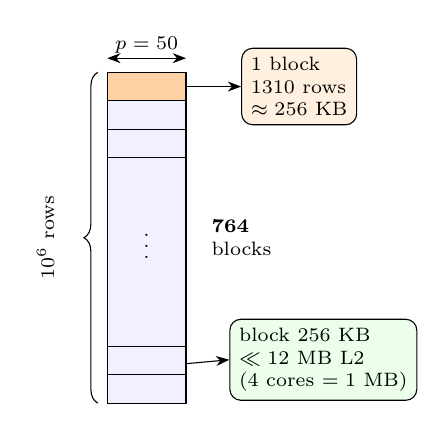
\begin{tikzpicture}[font=\scriptsize, >=Stealth]
      \def\w{1.0}\def\h{4.2}
      % the matrix X
      \draw[fill=blue!6] (0,0) rectangle (\w,\h);
      % top three block dividers + highlight the first block
      \fill[orange!35] (0,\h-0.36) rectangle (\w,\h);
      \draw (0,\h-0.36) rectangle (\w,\h);
      \draw (0,\h-0.72)--(\w,\h-0.72);
      \draw (0,\h-1.08)--(\w,\h-1.08);
      % bottom two dividers
      \draw (0,0.36)--(\w,0.36);
      \draw (0,0.72)--(\w,0.72);
      \node at (\w/2,\h/2) {$\vdots$};
      % width label
      \draw[<->] (0,\h+0.18)--(\w,\h+0.18);
      \node[above] at (\w/2,\h+0.12) {$p=50$};
      % height brace
      \draw[decorate,decoration={brace,amplitude=5pt,mirror}] (-0.12,\h)--(-0.12,0);
      \node[rotate=90,anchor=south] at (-0.55,\h/2) {$10^{6}$ rows};
      % callout: one block
      \node[draw,rounded corners,fill=orange!12,align=left,anchor=west]
        (blk) at (\w+0.7,\h-0.18) {1 block\\ $1310$ rows\\ $\approx 256$ KB};
      \draw[->] (\w,\h-0.18) -- (blk.west);
      % total blocks
      \node[anchor=west,align=left] at (\w+0.2,\h/2) {$\mathbf{764}$\\ blocks};
      % L2 fit box
      \node[draw,rounded corners,fill=green!8,align=left,anchor=west]
        (l2) at (\w+0.55,0.55) {block $256$ KB\\ $\ll 12$ MB L2\\ (4 cores $=1$ MB)};
      \draw[->] (\w,0.5) -- (l2.west);
    \end{tikzpicture}
  \end{columns}
\end{frame}

\begin{frame}[fragile]{Fused Pass Implementation}
\begin{lstlisting}
let dots: Vec<f32> = x_raw
    .par_chunks(block_rows * n_cols)          // one block per task
    .zip(r.par_chunks_mut(block_rows))        // matching residual slice
    .fold(|| vec![0.0f32; n_cols], |mut local_dots, (x_block, r_block)| {
        // Phase 1: bring r[block] in sync with coef_prev
        for (row, ri) in x_block.chunks(n_cols).zip(r_block.iter_mut()) {
            *ri -= dot_scalar(row, &prev_deltas);   // X cold -> L2
        }
        // Phase 2: accumulate X^T r  (X L2-hot, r L1-hot)
        for (row, &ri) in x_block.chunks(n_cols).zip(r_block.iter()) {
            axpy_scalar(&mut local_dots, ri, row);
        }
        local_dots
    })
    .reduce(|| vec![0.0f32; n_cols],
            |mut a, b| { for j in 0..n_cols { a[j] += b[j] } a });
\end{lstlisting}
\end{frame}

\begin{frame}[fragile]{The Intercept Lag Problem}
  Because phase~1 applies $\Delta w_{\text{prev}}$ (not $\Delta w_{\text{cur}}$),
  after the fused pass $r$ still reflects the \emph{previous} coefficients.

  \vspace{0.4em}
  \textbf{Exact correction} using column sums $c_j = \sum_i X_{ij}$ (precomputed once):
  \[
    \Delta b = \frac{\sum_i r_i}{n} - \frac{c^\top \Delta w_{\text{cur}}}{n}
  \]
\begin{lstlisting}
let lag: f32 = col_sum.iter().zip(prev_deltas.iter())
                       .map(|(&s, &d)| s * d).sum::<f32>();
let b_delta  = r.iter().sum::<f32>() / n - lag / n;
intercept   += b_delta;
for ri in r.iter_mut() { *ri -= b_delta; }
\end{lstlisting}
  \vspace{0.2em}
  \texttt{col\_sum} is $O(np)$ to compute but paid only once; per-iteration cost is $O(p)$.
\end{frame}

\begin{frame}[fragile]{Thread Pool Integration}
  All parallel work is routed through the \emph{stratum global thread pool}:
  \begin{itemize}
    \item Controlled by \texttt{SKRUB\_RUST\_THREADS} / \texttt{num\_threads} config
    \item \texttt{get\_thread\_pool()} returns \texttt{Some(pool)} or \texttt{None}
    \item \texttt{None} $\Rightarrow$ Rayon's default global pool (one thread per core)
  \end{itemize}
  \vspace{0.4em}
\begin{lstlisting}
let pool = get_thread_pool();
// ...
match pool { Some(p) => p.install(compute), None => compute() }
\end{lstlisting}
  \vspace{0.4em}
  This ensures the Rust extension never fights with other parallel workloads
  (e.g.\ NumPy's BLAS threads) for CPU time.
\end{frame}

% ─────────────────────────────────────────────────────────────────────────────
\section{Commit 3 — Predict Optimisations and Benchmark Tiers}

\begin{frame}{Predict: Two Hidden Costs Fixed}
  \begin{columns}
    \column{0.5\textwidth}
    \textbf{Before (commit 1 predict)}
    \begin{itemize}
      \item Accepted \texttt{Array2<f32>} by value $\Rightarrow$ full matrix copy across FFI boundary
      \item One Rayon task per row $\Rightarrow$ scheduling overhead dominated for wide matrices
      \item Result: predict \emph{slower} than sklearn at scale
    \end{itemize}
    \column{0.5\textwidth}
    \textbf{After (commit 3 predict)}
    \begin{itemize}
      \item Accept \texttt{ArrayView2<f32>} — zero-copy borrow through PyO3
      \item Rows grouped into $\sim$256 KB blocks matching L2 cache — same block size as fit
      \item Result: $\sim$9--11$\times$ faster than sklearn; no superlinear blowup
    \end{itemize}
  \end{columns}
\end{frame}

\begin{frame}[fragile]{Zero-Copy Predict Signature}
  \textbf{Before} — takes ownership, forces memcpy at FFI boundary:
\begin{lstlisting}
pub fn elastic_net_predict(x: Array2<f32>, ...) -> ...
\end{lstlisting}

  \textbf{After} — borrows a view, read-only, zero allocation:
\begin{lstlisting}
pub fn elastic_net_predict(x: ArrayView2<f32>, ...) -> Result<Vec<f32>, String>
\end{lstlisting}
  \vspace{0.4em}
  The PyO3 binding passes \texttt{x.as\_array()} — a non-owning view into the
  existing numpy buffer.  No copy, no extra heap allocation.
\end{frame}

\begin{frame}[fragile]{Block-Parallel Predict}
\begin{lstlisting}
let block_rows = (256_usize * 1024 / (n_cols * 4)).clamp(64, 4096);
let mut preds  = vec![0.0f32; n_rows];
let mut compute = || {
    raw.par_chunks(block_rows * n_cols)
       .zip(preds.par_chunks_mut(block_rows))
       .for_each(|(x_block, p_block)| {
           for (row, p) in x_block.chunks(n_cols).zip(p_block.iter_mut()) {
               *p = dot_scalar(row, coef) + intercept;
           }
       });
};
match pool { Some(p) => p.install(compute), None => compute() };
\end{lstlisting}
  Each block is large enough that Rayon's steal overhead is negligible
  and the inner loop stays in L2.
\end{frame}

\begin{frame}{Benchmark Tiers}
  Commit 3 extended the benchmark with three mutually exclusive size tiers:

  \vspace{0.4em}
  \begin{center}
  \begin{tabular}{llrr}
    \hline
    \textbf{Flag} & \textbf{Label} & \textbf{Rows} & \textbf{Memory} \\
    \hline
    (default) & small / medium & up to $100{,}000$ & $\lesssim$50 MB \\
    \texttt{--large}   & large          & $500{,}000$       & $\sim$200 MB \\
    \texttt{--xlarge}  & extra-large    & $1{,}000{,}000$   & $\sim$400 MB \\
    \texttt{--xxlarge} & xx-large       & $5{,}000{,}000$   & $\sim$2 GB  \\
    \hline
  \end{tabular}
  \end{center}

  \vspace{0.4em}
  \begin{itemize}
    \item \texttt{--no-sklearn} skips sklearn at very large sizes to avoid OOM
      from the implicit \texttt{f64} copies sklearn requires
    \item Fits and predicts reported separately so bottlenecks are visible per phase
  \end{itemize}
\end{frame}

% ─────────────────────────────────────────────────────────────────────────────
\section{Experimental Setup}

\begin{frame}{System Specifications}
  \begin{columns}[T]
    \column{0.52\textwidth}
    \textbf{Hardware — Apple MacBook Pro (M1, 2020)}
    \begin{itemize}
      \item SoC: \textbf{Apple M1} (5 nm), 8-core CPU
      \item \textbf{4 Firestorm P-cores} ($\leq$3.2 GHz) +
            \textbf{4 Icestorm E-cores} ($\leq$2.06 GHz)
      \item Cache line: \textbf{128 B} (32 \texttt{f32} / 16 \texttt{f64})
      \item P-core: 128 KB L1d, 192 KB L1i, \textbf{12 MB shared L2}
      \item E-core: 64 KB L1d, \textbf{4 MB shared L2}; $\sim$8 MB System-Level
            Cache (no monolithic L3)
      \item \textbf{8 GB} unified LPDDR4X-4266 ($\sim$68 GB/s)
    \end{itemize}
    \column{0.48\textwidth}
    \textbf{Software}
    \begin{itemize}
      \item macOS 26.5.1 (build 25F80)
      \item Python 3.13 · NumPy 2.3.4 · scikit-learn 1.8.0
      \item Rust extension via PyO3 / maturin, \texttt{--release}
            (\texttt{opt-level=3}), Rayon thread pool
    \end{itemize}
    \vspace{0.3em}
    \begin{alertblock}{Why 8 GB RAM matters}
      The XX-Large case is $10^7\times50$: \texttt{f32} $=$ 2 GB, sklearn's
      \texttt{f64} copy $=$ 4 GB. On an 8 GB machine that alone drives sklearn
      into memory pressure — a real contributor to its 291 s fit.
    \end{alertblock}
  \end{columns}
\end{frame}

\begin{frame}{Run Configuration}
  \begin{columns}[T]
    \column{0.5\textwidth}
    \textbf{ElasticNet hyper-parameters (fit)}
    \begin{center}\small
    \begin{tabular}{ll}
      \hline
      Parameter & Value \\
      \hline
      \texttt{alpha} ($\alpha$)      & \texttt{0.1} \\
      \texttt{l1\_ratio} ($\rho$)    & \texttt{0.5} (equal L1/L2) \\
      \texttt{max\_iter}             & \texttt{1000} \\
      \texttt{tol}                   & \texttt{1e-4} \\
      \texttt{fit\_intercept}        & \texttt{True} \\
      \hline
    \end{tabular}
    \end{center}
    \vspace{0.3em}
    \textbf{Correctness runs} tighten this to \texttt{max\_iter=10000},
    \texttt{tol=1e-6}, accepted at \texttt{rtol=5\%}.
    \vspace{0.4em}
    \textbf{Predict}
    \begin{itemize}
      \item $\hat{y} = Xw + b$ on the \emph{training} $X$
      \item Same fitted model reused across timing reps
    \end{itemize}
    \column{0.5\textwidth}
    \textbf{Data (synthetic, seed $=$ 42)}
    \begin{itemize}
      \item $X \sim \mathcal{N}(0,1)^{n\times p}$
      \item true $w \sim \mathcal{N}(0,1)^{p}$
      \item $y = Xw + 0.1\,\mathcal{N}(0,1)$
    \end{itemize}
    \vspace{0.4em}
    \textbf{Data types}
    \begin{itemize}
      \item \textbf{Rust: \texttt{f32}}, C-contiguous (row-major)
      \item \textbf{sklearn: \texttt{f64}} (its solver upcasts internally)
      \item Identical $X, y$ values fed to both
    \end{itemize}
    \vspace{0.4em}
    \textbf{Timing protocol}
    \begin{itemize}
      \item Median of 5 reps (3 for $\geq$2 GB), 2 warm-ups discarded
      \item \texttt{gc.collect()} before each rep
      \item Each cell in its own subprocess (thread-pool isolation)
    \end{itemize}
  \end{columns}
\end{frame}

\begin{frame}[fragile]{Memory Layout and Iteration Order}
  \begin{columns}[T]
    \column{0.5\textwidth}
    \textbf{Row-major (C-contiguous) throughout}
    \begin{itemize}
      \item $X$ is taken exactly as NumPy stores it — row-major \texttt{f32},
            \textbf{no transpose, no copy}
      \item The fit loop streams $X$ in contiguous row-blocks:
    \end{itemize}
\begin{lstlisting}
x_raw.par_chunks(block_rows * n_cols)   // contiguous block
     ...
     for row in x_block.chunks(n_cols)  // row by row
\end{lstlisting}
    \begin{itemize}
      \item Every inner \texttt{dot}/\texttt{axpy} walks a row's $p$ elements at
            \textbf{unit stride} $\Rightarrow$ full 128 B cache lines, hardware
            prefetcher stays locked on
    \end{itemize}
    \column{0.5\textwidth}
    \textbf{Why row-major, when CD is "column-oriented"}
    \begin{itemize}
      \item Classic cyclic CD updates one \emph{feature} (column) at a time and
            needs column-contiguous data — sklearn therefore requires/copies to
            \textbf{Fortran order} (column-major)
      \item Our Jacobi reformulation accumulates $X^\top r$ by an \texttt{axpy}
            into a per-column accumulator \emph{while streaming rows}, converting
            strided column access into \textbf{sequential row access}
      \item So we get unit-stride traffic \emph{and} skip sklearn's F-order copy
    \end{itemize}
    \vspace{0.3em}
    \textbf{Block sizing}
    \begin{itemize}
      \item Target 256 KB of $X$ per Rayon task, clamped to $[64, 4096]$ rows —
            keeps each thread's block + residual hot in L1/L2
      \item Predict reuses the same row-block streaming over a zero-copy
            \texttt{ArrayView2} borrow
    \end{itemize}
  \end{columns}
\end{frame}

% ─────────────────────────────────────────────────────────────────────────────
\section{Benchmark Results}

\begin{frame}{Benchmark Methodology}
  \begin{columns}[T]
    \column{0.52\textwidth}
    \textbf{What is measured}
    \begin{itemize}
      \item HEAD (block-parallel) Rust vs.\ sklearn \texttt{ElasticNet}
      \item Four size tiers, from $10^4$ to $10^7$ rows
      \item Thread counts 1, 2, 4, 8 (machine has 8 cores)
      \item Median of 5 reps (3 for the largest); 2 warm-up runs discarded
      \item \texttt{f32} matrix for Rust, \texttt{f64} for sklearn,
            $\alpha{=}0.1$, $\rho{=}0.5$, \texttt{max\_iter}{=}1000
    \end{itemize}
    \column{0.48\textwidth}
    \textbf{Reproducibility \& correctness}
    \begin{itemize}
      \item All timings cached in \texttt{elastic\_net\_full\_cache.json};
            each cell runs in an isolated subprocess so the thread pool
            initialises with the right count
      \item Charts regenerated from the cache by
            \texttt{plot\_bar\_charts.py} and
            \texttt{plot\_thread\_comparison.py}
      \item Every commit verified vs.\ sklearn at \texttt{rtol=5\%},
            \texttt{tol=1e-6}, 10k iterations — predictions agree to
            $<0.2\%$ despite \texttt{f32}
    \end{itemize}
  \end{columns}
\end{frame}

\begin{frame}{Rust vs Sklearn — Small and Large Inputs (8 threads)}
  \begin{center}
    \includegraphics[width=\textwidth, height=0.80\textheight, keepaspectratio]%
      {benchmarks/results/elastic_net_bars_small_large.png}
  \end{center}
  \vspace{-0.5em}
  {\footnotesize
    Solid = fit, hatched = predict · log $y$-axis · label above each Rust bar =
    speedup over sklearn}
\end{frame}

\begin{frame}{Rust vs Sklearn — X-Large and XX-Large Inputs (8 threads)}
  \begin{center}
    \includegraphics[width=\textwidth, height=0.80\textheight, keepaspectratio]%
      {benchmarks/results/elastic_net_bars_xlarge_xxlarge.png}
  \end{center}
  \vspace{-0.5em}
  {\footnotesize
    At 10M$\times$50 sklearn fit takes $\sim$291 s vs.\ $\sim$2.3 s for Rust —
    a $129\times$ gap at 8T (and $222\times$ at 2T)}
\end{frame}

\begin{frame}{Why Speedup Grows With Data Size}
  \begin{columns}[T]
    \column{0.5\textwidth}
    \textbf{The trend (fit speedup over sklearn)}
    \begin{center}\small
    \begin{tabular}{lcc}
      \hline
      Size & 1 thread & best \\
      \hline
      100k$\times$50 (20 MB)  & $3.6\times$ & $8.8\times$ \\
      500k$\times$50 (100 MB) & $4.0\times$ & $10.3\times$ \\
      2M$\times$50 (400 MB)   & $7.6\times$ & $20.8\times$ \\
      10M$\times$50 (2 GB)    & $116\times$ & $222\times$ \\
      \hline
    \end{tabular}
    \end{center}
    \vspace{0.3em}
    Speedup climbs even at \emph{one thread} — so this is not merely parallelism.

    \column{0.5\textwidth}
    \textbf{Three compounding reasons}
    \begin{itemize}
      \item \textbf{Fixed costs amortise}: Python$\leftrightarrow$Rust FFI,
            thread-pool spin-up and warm-up are constant — negligible at 10M
            rows, a large fraction at 10k.
      \item \textbf{\texttt{f32} cache edge compounds}: sklearn's \texttt{f64}
            working set is $2\times$ ours, so it outgrows each cache level
            sooner and thrashes DRAM harder as data grows.
      \item \textbf{sklearn's superlinear wall}: its fit jumps
            $1.3\,\text{s}\!\to\!291\,\text{s}$ for $5\times$ the data
            ($217\times$). A 4 GB \texttt{f64} working set dwarfs every cache
            \emph{and} nearly fills the 8 GB RAM — near-total cache misses plus
            memory pressure, and more sweeps to converge. Our \texttt{f32} fused
            single-pass halves the footprint and converges in a few iterations.
    \end{itemize}
  \end{columns}
\end{frame}

% ─────────────────────────────────────────────────────────────────────────────
\begin{frame}{Runtime vs Thread Count — Small and Large}
  \begin{center}
    \includegraphics[width=\textwidth, height=0.80\textheight, keepaspectratio]%
      {benchmarks/results/elastic_net_thread_comparison_small_large.png}
  \end{center}
  \vspace{-0.5em}
  {\footnotesize
    HEAD runtime (log ms) vs thread count · dashed/dotted lines = sklearn
    fit/predict · label above each bar = speedup over sklearn}
\end{frame}

\begin{frame}{Runtime vs Thread Count — X-Large and XX-Large}
  \begin{center}
    \includegraphics[width=\textwidth, height=0.80\textheight, keepaspectratio]%
      {benchmarks/results/elastic_net_thread_comparison_xlarge_xxlarge.png}
  \end{center}
  \vspace{-0.5em}
  {\footnotesize
    Note the XX-Large fit \emph{minimum at 2 threads} ($222\times$) — adding
    cores past 2 makes it \emph{slower}}
\end{frame}

\begin{frame}{Why the Thread-Count Trends}
  \begin{columns}[T]
    \column{0.5\textwidth}
    \textbf{1T $\to$ 4T: near-linear gains}
    \begin{itemize}
      \item Each 256 KB row block gives a thread enough work to hide Rayon
            steal/barrier latency
      \item Larger inputs scale better — more blocks per thread amortise the
            fixed per-pass overhead
    \end{itemize}
    \vspace{0.3em}
    \textbf{4T $\to$ 8T: plateau}
    \begin{itemize}
      \item Apple Silicon = 4 performance + 4 efficiency cores
      \item Fit is memory-bandwidth bound; 4 P-cores already saturate the DRAM
            channels, so E-cores add scheduling cost without bandwidth
      \item Small inputs can even \emph{regress} at 8T: too few blocks to feed
            8 threads, steal overhead $>$ useful work
    \end{itemize}

    \column{0.5\textwidth}
    \textbf{XX-Large fit inverts: 2T is best}
    \begin{itemize}
      \item At a 2 GB working set the fused pass is \emph{purely}
            DRAM-bandwidth bound
      \item Past 2 threads the extra cores contend for the same memory
            controllers (and pull in slower E-cores):
            $222\times$ at 2T $\to$ $129\times$ at 4T/8T
      \item Lesson: for huge memory-bound fits, fewer threads can be faster
    \end{itemize}
    \vspace{0.3em}
    \textbf{Predict scales more cleanly}
    \begin{itemize}
      \item Embarrassingly parallel — no sequential $O(p)$ coordinate reduction
      \item Keeps improving with threads at large sizes (subject to noise)
    \end{itemize}
  \end{columns}
\end{frame}

% ─────────────────────────────────────────────────────────────────────────────
\section{Benchmark Takeaways}

\begin{frame}{Speedup Summary and Practical Guidance}
  \begin{columns}[T]
    \column{0.52\textwidth}
    \textbf{Speedup over sklearn (best thread count)}
    \begin{center}\small
    \begin{tabular}{lcc}
      \hline
      Size & fit & predict \\
      \hline
      100k$\times$50 (20 MB)  & $8.8\times$  & $4.0\times$ \\
      500k$\times$50 (100 MB) & $10.3\times$ & $4.3\times$ \\
      2M$\times$50 (400 MB)   & $20.8\times$ & $4.6\times$ \\
      10M$\times$50 (2 GB)    & $222\times$  & $7.9\times$ \\
      \hline
    \end{tabular}
    \end{center}
    \vspace{0.3em}
    Both phases beat sklearn at every size; the fit advantage explodes as the
    problem outgrows cache.

    \column{0.48\textwidth}
    \textbf{Rules of thumb}
    \begin{itemize}
      \item \textbf{Threads}: 4 is the sweet spot for most sizes; use 2 for
            multi-GB fits, and 8 only when predict-bound
      \item \textbf{Fit} is memory-bandwidth bound — the \texttt{f32} + fused
            single-pass wins \emph{grow} with data size
      \item \textbf{Predict} is compute-bound and embarrassingly parallel —
            steady $4$–$8\times$, best at high thread counts
      \item Single-thread already beats sklearn, so the gains are algorithmic
            (\texttt{f32}, fused pass) \emph{and} parallel — not parallelism alone
    \end{itemize}
  \end{columns}
\end{frame}

% ─────────────────────────────────────────────────────────────────────────────
\section{What Makes This Fast}

\begin{frame}{Four Orthogonal Optimisations}
  The overall speedup is the product of four independent techniques.
  Each addresses a different bottleneck; removing any one degrades performance
  significantly.

  \vspace{0.6em}
  \begin{center}
  \begin{tabular}{clp{6cm}}
    \hline
    \textbf{\#} & \textbf{Technique} & \textbf{Primary effect} \\
    \hline
    1 & \texttt{f32} over \texttt{f64}    & 2$\times$ SIMD width, 2$\times$ less DRAM traffic \\
    2 & Rayon parallelism (Jacobi CD)     & near-linear fit scaling to 4--8 threads \\
    3 & Cache-fused single pass           & halved DRAM reads for $X \gtrsim 20$ MB \\
    4 & Block tiling + zero-copy FFI      & eliminates scheduling overhead and memcpy \\
    \hline
  \end{tabular}
  \end{center}

  \vspace{0.6em}
  \begin{block}{Observed cumulative effect}
    \textbf{Fit}: up to $10\times$ faster than sklearn at 500k rows \\
    \textbf{Predict}: up to $12\times$ faster at 100k rows with 8 threads
  \end{block}
\end{frame}

\begin{frame}[fragile]{\#1 — \texttt{f32} Precision: Half the Data, Twice the SIMD}
  \begin{columns}[T]
    \column{0.48\textwidth}
    \textbf{Why sklearn is slow here}
    \begin{itemize}
      \item sklearn calls \texttt{ElasticNet} which uses \texttt{float64} internally
      \item Every memory access and SIMD lane operates on 8-byte values
      \item A $100{,}000 \times 50$ matrix = 40 MB in \texttt{f64}, 20 MB in \texttt{f32}
    \end{itemize}
    \vspace{0.5em}
    \textbf{What \texttt{f32} buys us}
    \begin{itemize}
      \item \textbf{2$\times$ more SIMD lanes}: 4 floats/register (SSE) or 8 (AVX2)
            vs.\ 2 or 4 doubles
      \item \textbf{2$\times$ less memory bandwidth}: smaller matrix $\Rightarrow$
            more of $X$ fits in each cache level
      \item \textbf{2$\times$ fewer cache misses}: same L2/SLC holds twice as many rows
    \end{itemize}

    \column{0.48\textwidth}
    \textbf{Precision trade-off}
    \begin{itemize}
      \item \texttt{f32} gives $\sim$7 decimal digits vs.\ $\sim$15 for \texttt{f64}
      \item Verified: max relative prediction error $< 0.18\%$ vs.\ sklearn \texttt{f64}
            at tight tolerance (\texttt{tol=1e-6}, 10k iterations)
      \item Coefficient MSE $\sim 10^{-14}$ — effectively identical solutions
      \item For regression predictions, \texttt{f32} accuracy is more than sufficient
    \end{itemize}

    \vspace{0.4em}
    \textbf{Single-thread fit already $2$--$3.6\times$ sklearn}\\
    The \texttt{f32} advantage is visible even before any parallelism is added.
  \end{columns}
\end{frame}

\begin{frame}{\#2 — Rayon Parallelism via Jacobi Coordinate Descent}
  \begin{columns}[T]
    \column{0.48\textwidth}
    \textbf{Why Jacobi enables parallelism}
    \begin{itemize}
      \item Jacobi CD freezes $w^{(t)}$ and computes \emph{all} $\Delta w_j$
            from the same residual snapshot
      \item Every row of $X$ contributes independently to the residual update
            and to $X^\top r$ — no inter-row data dependency
      \item This makes the inner loop \textbf{embarrassingly parallel}:
            Rayon tasks never share mutable state within a pass
    \end{itemize}
    \vspace{0.4em}
    \textbf{Only 2 barriers per outer iteration}
    \begin{itemize}
      \item 1 barrier after the fused pass (collect \texttt{dots})
      \item 1 barrier after the coordinate update (broadcast \texttt{prev\_deltas})
      \item Gauss-Seidel would require $2p$ barriers ($p =$ number of features)
    \end{itemize}

    \column{0.48\textwidth}
    \textbf{Rayon work-stealing scheduler}
    \begin{itemize}
      \item \texttt{par\_chunks} divides the row range into equal segments;
            idle threads steal tasks from the back of busy threads' queues
      \item No manual load-balancing needed — Rayon adapts to heterogeneous
            core speeds (P-cores vs.\ E-cores on Apple Silicon)
    \end{itemize}
    \vspace{0.4em}
    \textbf{Observed scaling (fit)}
    \begin{center}
    \small
    \begin{tabular}{rcc}
      \hline
      Threads & 20 MB & 40 MB \\
      \hline
      1T & 1.0$\times$ & 1.0$\times$ \\
      2T & 1.5$\times$ & 1.8$\times$ \\
      4T & 2.4$\times$ & 2.7$\times$ \\
      8T & 2.4$\times$ & 2.7$\times$ \\
      \hline
    \end{tabular}
    \end{center}
    \vspace{0.2em}
    {\footnotesize 4T $\approx$ 8T: memory bus saturated; E-cores add overhead.}
  \end{columns}
\end{frame}

\begin{frame}{\#3 — Cache-Fused Single Pass: One Read of $X$ Per Iteration}
  \textbf{The original two-pass bottleneck for large $X$}

  \vspace{0.3em}
  When $X$ exceeds L3 ($\gtrsim$20 MB on most CPUs), each pass reads $X$
  entirely from DRAM.  The two-pass algorithm therefore spends
  $2 \times n \times p \times 4$ bytes of DRAM bandwidth per iteration.

  \vspace{0.6em}
  \textbf{Cache-fusion principle}
  \begin{enumerate}
    \item Each Rayon task claims a $\sim$256 KB \emph{block} of $X$ rows
          (fits in L2 cache)
    \item \textbf{Phase 1}: load block from DRAM $\to$ L2; update $r[\text{block}]$
          using $\Delta w_{\text{prev}}$
    \item \textbf{Phase 2}: accumulate $X[\text{block}]^\top r[\text{block}]$
          while the block is still \textbf{L2-hot} (no DRAM access)
    \item Task releases the block; moves to the next one
  \end{enumerate}

  \vspace{0.4em}
  \begin{columns}
    \column{0.5\textwidth}
    \textbf{Result}
    \begin{itemize}
      \item $n \times p \times 4$ bytes / iteration — \textbf{half the DRAM traffic}
      \item Measurable improvement begins once $X$ outgrows the last cache level
      \item On the M1 (12 MB P-cluster L2 + $\sim$8 MB SLC, no true L3) the gain
            appears at $\gtrsim$20 MB; on x86 with 8--16 MB shared L3 it appears
            in the same range and is $1.5$--$2\times$
    \end{itemize}
    \column{0.5\textwidth}
    \textbf{Why this works}
    \begin{itemize}
      \item $r[\text{block}]$ fits in L1 after phase 1 (tiny compared to $X$)
      \item L2 block lifetime matches both phase 1 and phase 2 read windows
      \item No extra memory required: operates in-place on the existing $r$ buffer
    \end{itemize}
  \end{columns}
\end{frame}

\begin{frame}[fragile]{\#4 — Block Tiling and Zero-Copy FFI}
  \begin{columns}[T]
    \column{0.48\textwidth}
    \textbf{Block tiling — why task granularity matters}
    \begin{itemize}
      \item Commit 1 predict: one Rayon task per \emph{row} (one dot product)
      \item Rayon's task-steal overhead is $\sim$0.5--2 $\mu$s per steal;
            a single dot product on a 50-column row takes $\sim$10 ns
      \item Result: scheduling overhead $\gg$ compute $\Rightarrow$ slower than sklearn at large $p$
    \end{itemize}
    \vspace{0.4em}
    \textbf{Fix: process rows in 256 KB blocks}
\begin{lstlisting}
let block_rows =
  (256 * 1024 / (n_cols * 4))
  .clamp(64, 4096);
\end{lstlisting}
    \begin{itemize}
      \item Each task does thousands of dot products — steal overhead is $< 0.1\%$
      \item Block size adapts automatically to $p$ at runtime
    \end{itemize}

    \column{0.48\textwidth}
    \textbf{Zero-copy FFI — eliminating the memcpy}

    PyO3 (the Python--Rust bridge) originally required passing $X$ by value:
\begin{lstlisting}
// Before: full matrix copy
fn predict(x: Array2<f32>)
// After: borrow the numpy buffer
fn predict(x: ArrayView2<f32>)
\end{lstlisting}
    \begin{itemize}
      \item \texttt{Array2} by value: PyO3 allocates a new $n \times p$ Rust array
            and copies the numpy data — $O(np)$ work before predict even starts
      \item \texttt{ArrayView2} borrows the existing numpy buffer read-only —
            zero allocation, zero copy
      \item At 200 MB matrix: saves $\sim$50 ms per call from the copy alone
      \item Combined with block tiling: predict goes from $< 1\times$ to $9$--$12\times$
            vs.\ sklearn
    \end{itemize}
  \end{columns}
\end{frame}

% ─────────────────────────────────────────────────────────────────────────────
\section{Algorithm Summary}

\begin{frame}{Full Algorithm Pipeline}
  \begin{enumerate}
    \item \textbf{Precompute} $\tfrac{1}{n}\|X_{:j}\|^2$ for all $j$ (parallel fold/reduce)
    \item \textbf{Precompute} $c_j = \sum_i X_{ij}$ for intercept correction (parallel)
    \item \textbf{Initialise} $w=0$, $b=\bar{y}$, $r = y - b$, $\Delta w_{\text{prev}}=0$
    \item \textbf{Iterate} until convergence or \texttt{max\_iter}:
    \begin{enumerate}
      \item \textbf{Fused pass} (parallel, one read of $X$):
            update $r$ with $\Delta w_{\text{prev}}$, then accumulate $X^\top r$
      \item \textbf{Coordinate update} (sequential, $O(p)$):
            apply soft-threshold, record $\Delta w_{\text{cur}}$
      \item \textbf{Intercept update} (sequential):
            exact lag correction using $c$ and $\Delta w_{\text{cur}}$
      \item \textbf{Convergence check}: $\max_j |\Delta w_j| / \max(|w_j|, 1) < \varepsilon$
    \end{enumerate}
    \item \textbf{Predict} $\hat{y} = Xw + b$ (parallel, zero-copy, block-tiled)
  \end{enumerate}
\end{frame}

\begin{frame}{Performance Characteristics}
  \begin{columns}
    \column{0.5\textwidth}
    \textbf{Complexity per iteration}
    \begin{itemize}
      \item Fused pass: $O(np)$ — one read of $X$
      \item Coordinate update: $O(p)$
      \item Intercept: $O(n + p)$
    \end{itemize}
    \vspace{0.4em}
    \textbf{Memory traffic (vs.\ two-pass)}
    \begin{itemize}
      \item Two-pass: $2 \times np \times 4$ B / iter
      \item Fused: $np \times 4$ B / iter
      \item \textbf{Halved DRAM bandwidth} for $X \gtrsim 20$ MB
    \end{itemize}
    \column{0.5\textwidth}
    \textbf{Observed speedups}
    \begin{itemize}
      \item Fit: 2--7$\times$ vs.\ sklearn (commit 1)
      \item Predict: 9--11$\times$ vs.\ sklearn (commit 3)
      \item Fit further improved by fused pass (commit 2) for large $X$
    \end{itemize}
    \vspace{0.4em}
    \textbf{Thread safety}
    \begin{itemize}
      \item All Rayon work runs inside \texttt{stratum} global pool
      \item No contention with BLAS / other extensions
    \end{itemize}
  \end{columns}
\end{frame}

% ─────────────────────────────────────────────────────────────────────────────

\begin{frame}{Summary of Commits}
  \begin{center}
  \begin{tabular}{lp{8.5cm}}
    \hline
    \textbf{Commit} & \textbf{Contribution} \\
    \hline
    \texttt{cdeb7a3} &
      Jacobi parallel CD: 2 barriers/iter, \texttt{par\_chunks} fold/reduce,
      PyO3 bindings, tests, benchmark. \\[4pt]
    \texttt{0ad4263} &
      Fused single-pass: halves DRAM traffic for large $X$; exact intercept
      lag correction via $c^\top \Delta w$; thread-pool integration. \\[4pt]
    \texttt{10f16bd} &
      Zero-copy \texttt{ArrayView2} predict; block-parallel rows; benchmark
      size tiers (\texttt{--large/--xlarge/--xxlarge}) and \texttt{--no-sklearn}. \\
    \hline
  \end{tabular}
  \end{center}
\end{frame}

\end{document}
